\section{Authorlists Acknowledgements and ProofChecker}
\label{sec:Authorlists_Acknowledgements_and_ProofChecker}

\subsection{Author lists and acknowledgments files}
\label{sec:Author_lists_and_acknowledgments_files}

Both types of files, author list and acknowledgements, are built using FENCE framework, see Fig.~\ref{fig:authorlist_interface}, and automatically pushed into the appropriate Gitlab repository, thanks to the FENCE Gitlab integration (chapter 6.3). Their implementation into the Paper is straightforward for a future submission to the journals. FENCE provides an elegant way to retrieve the needed information from the database (see chapter 4.5 MBF infrastructure) and build all the needed files.
 
The Author lists XML file is composed by three main blocks:
\begin{itemize}
\item Header: store paper main information (\ref{sec:app10})
\item Institutes: list of institutes and their references (\ref{sec:app11})
\item Authors: list of authors for this author list with their information (\ref{sec:app12})
\end{itemize}
 
XML file is the one used as a “role” since it contains all the information needed to build the other files. It is the first one to be generated and a backup version of the first release of the author list is stored.
 
The acknowledgment TEX file is built using a standard template and it is filled using the FENCE framework to retrieve the needed information about the ATLAS Founding Agencies.

\begin{figure}[ht!]
  \centering
  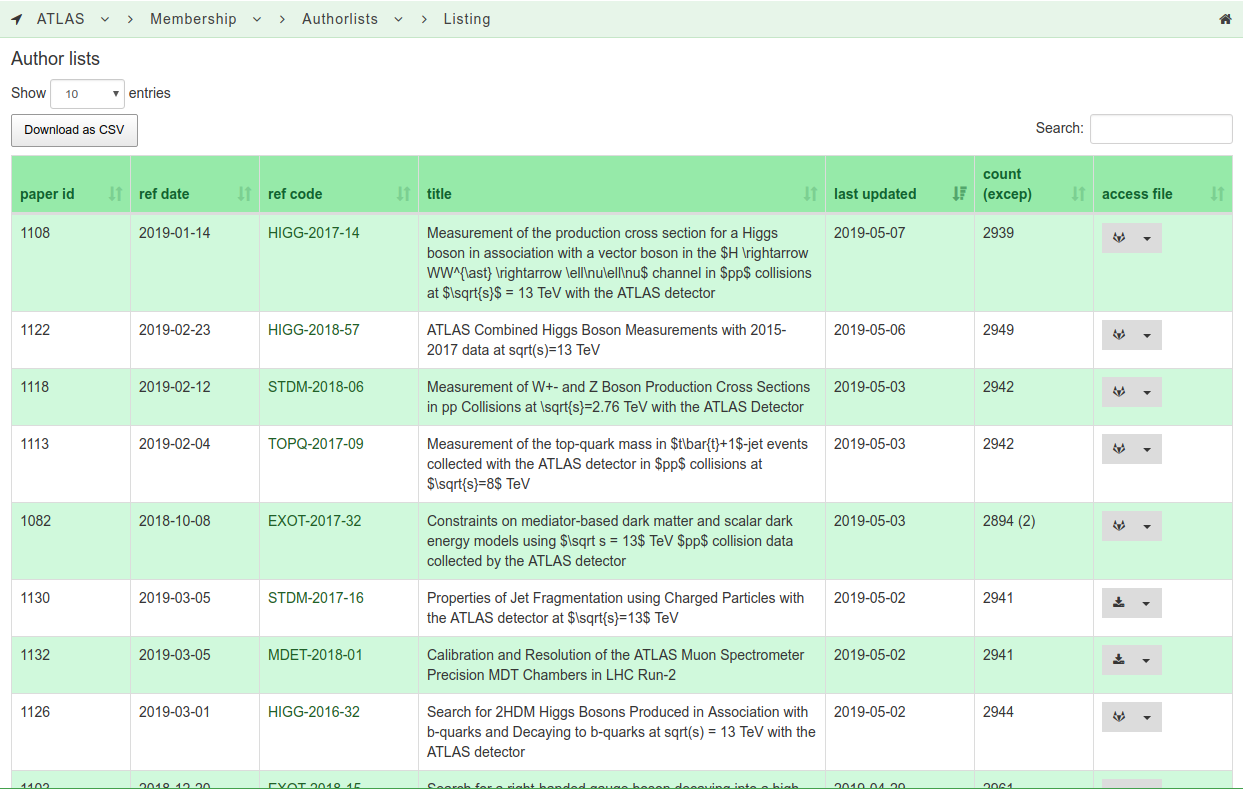
\includegraphics[width=0.9\textwidth]{figures/authorlist_interface.png}
  \caption{FENCE Authorlist interface. The five first in the list are GitLab projects.}
  \label{fig:authorlist_interface}
\end{figure}

\subsection{Main functionalities of the FENCE Author list user interface}
\label{sec:Main_functionalities_of_the_FENCE_Author_list_user_interface}

The FENCE Author list interface, Fig.~\ref{fig:authorlist_interface}, shows the complete set of author lists created for each ATLAS Paper which is published since 2009 or being submitted. They are easily filtered using the SEARCH box option. All the columns are self-explanatory; in the last column the dropdown menu gives access to the author list location, which can be distinguished by the icon: a download\textbf{ icon ()} means the files are stored in AFS and can be downloaded. A GitLab \textbf{icon ()} means the Paper and the files are located in a PO Gitlab repository. The author lists can be downloaded or displayed in Gitlab in different file formats (tex, xml, csv, pdf, cds) and structures (by country/institutes, or institutes only). 

\subsection{Proof checker functionalities}
\label{sec:Proof_checker_functionalities}
Once the author list is sent to the journal together with the publication, it’s time to check if the publisher correctly used the information provided by going through the journal pdf file sent to ATLAS Physics Office and comparing to the xml/tex file. This process, once done by hand, required the officer to verify if each author (~2800) and each institute (~200) is correctly reported and matched. 
For this purpose, a tool, the proof checker, was created to automatically poll the proof directories for new pdf documents uploaded. If it finds a document that has not been checked before, it starts the following process:

\begin{itemize}
\item Retrieves the information from the XML file created on Paper Submission Phase;
\item Extracts the text from the journal pdf file;
\item Parses the text from the pdf file, creating the target reference;
\item Compares the official reference obtained from the XML file with the target reference;
\item Creates a report with the differences found between the original and the target reference;
\item Links the report to the main report page, Fig.~\ref{fig:collaboration_proofs}.
\end{itemize}

\begin{figure}[ht!]
  \centering
  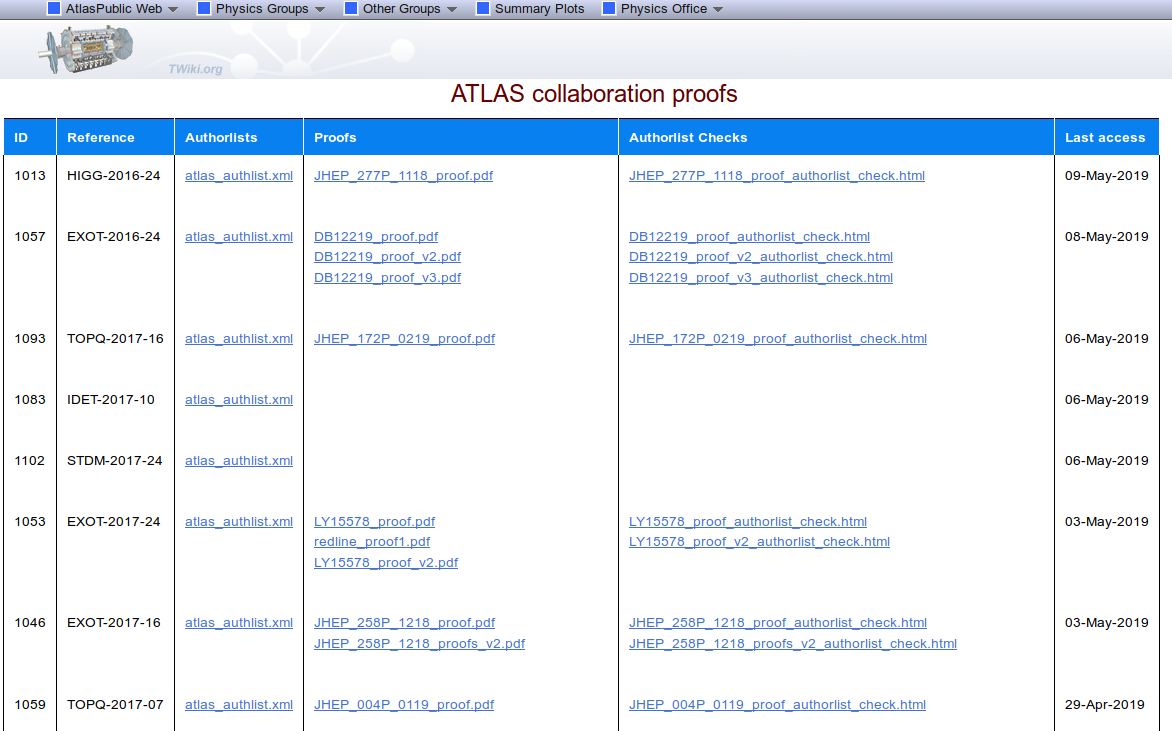
\includegraphics[width=0.9\textwidth]{figures/collaboration_proofs.png}
  \caption{Atlas collaboration proofs main page.}
  \label{fig:collaboration_proofs}
\end{figure}
The main difficulties in this process rely on extracting the content from the PDF file; the text is not easily retrieved for different reasons. 
One is that there are a lot of elements that have to be identified and ignored, such as row numbers, watermarks, footpages and headings. 
Another reason is that words extracted from a PDF file don’t follow a specific coding convention: other than ASCII characters can be output in many different ways; PDF can specify a predefined encoding to use, or provide a lookup table of differences to a predefined or built-in encoding; for fonts with non common latin characters, which is always the case for these kind of publications and content, special encodings are used and should be necessary to provide a ToUnicode table when semantic information about the characters has to be preserved. 
Also the proof checker has to pass through all the publication text and try to “understand” when the author list starts, when it ends, when the institute list starts and when it ends.
All this is made even more difficult due to the fact that different publishers have different layouts, and create different versions of PDF files, making all of the above problems not generic but often specific to themselves only.

After the target reference is created, the comparison looks for:

\begin{itemize}
\item Authors that seem to be missing from the PDF. Here, false positives are often due to characters encoding and spaces;
\item Authors with inconsistent punctuation. This section points out differences between original and target references authors’ first names punctuation to follow the rule X. or X.Y. or X.-Y. or X-Y. with no spaces at all.;
\item Institutes that seem missing from the PDF. Here false positives are often due to non standard characters which breaks the entry;
\item Institutes with close matches. All the entries that really look like the original but have some inconsistencies get in this group. Some publisher expands (or contracts) USA to United States of America, or there’s some new character which doesn’t break the institute entry but makes it so that there’s no perfect match, such as “Università” and “Universit` a”;
\item Mismatched authors. All the authors collaborate through one or more institutes. It is checked that the link between the author and the institute is consistent. This sometimes results as a false positive because it’s not always easy to extract from the pdf the index number of an institute, mainly because the text coming from the pdf file is often full of other elements such as line numbers of the document. For this reason an author originally assigned to institute number X, can result matched with target institute YX, because in the text extracted from the pdf the number X might be preceded by a Y line number; institute YX mostly doesn’t exist or eventually comes to be another institute;
\item Deceased authors. In two categories we show a list, often empty, of authors that we signed as deceased but the publication forgot to mark, or vice-versa. The results here are pretty reliable;
\item Missing founding agencies, or wrongly added by the publisher are checked.
\end{itemize}

In early 2019, due to some changes on CERN systems, the component written in PROLOG which run the comparison went out of service. This implied an urgent request for developing a new tool that could take care of this task. PROLOG is well known to take a different approach in a generic problem solving situation, where the expression of the problem is translated in a logic way instead of working directly on its resolution algorithm. But PROLOG is also a language difficult to maintain due to the fact that not many developers had ever a chance to work with it and its logic programming paradigm. That’s why python was chosen to accomplish this role.

The main issue was to find a way to get the best match among all the items of an array of institutes and authors because we can’t blindly rely on finding an author or institute in the same position of the sequence, and just compare author~1 on the xml file with author~1 in the pdf file and so on, as this is not always the case. For this purpose the concept of Levenshtein distance (\ref{sec:app16}) has been used, so that a weighted index of similarity could be obtained to “decide” what is matched with what, to then effectively start checking for anomalies.

At the end, a feature has been developed to help the script to evaluate as perfect matches some that wouldn’t otherwise. A list of “synonyms” is created for every entry, author or institute, to teach the proof checker to validate similar strings when the differences are due only to problems we have when decoding the text from the pdf file. So, for instance, if author \textbf{A. Filipčič} is not found in the target reference, but from the pdf entries we extracted an author with name \textbf{A. Filipž ciž c}, then, as it has been previously verified that in the pdf file the name appears as expected, the proof checker considers it a perfect match, and skips the problem. A very long list of false positives can be found in the report page as “skipped items”. The list of synonyms is updated manually, but a tool, the Synonym webpage (\ref{sec:Synonym_webpage}), has been created to allow users to update this list themselves.


\subsubsection{Proof checker synonyms}
\label{sec:Proof_checker_synonyms}
The comparison between PDF file (coming from the Journals) and the XML file (provided by FENCE author list interface) generates a lot of false positives as described in \ref{sec:Report_page}: special characters encoding can be different, countries sometimes are spelled differently, etc. To avoid having a huge list of these kind of false positives into the report page that can confuse the users, the new version of the proof checker includes a “synonyms” list that allows the comparison script to understand if the difference is a real error or another correct way to display the same information. An example of a working synonym is:
\begin{table}[ht!]
\centering
\begin{tabular}{|c|}
\hline
\textbf{Institute as stored into ATLAS DB \& XML file} \\
\hline
Physics Department, SUNY Albany, Albany NY, United States of America \\
\hline
\textbf{Institute as written on the journal’s author list} \\
\hline
Physics Department, SUNY Albany, Albany, New York, USA \\
\hline
\end{tabular}
\end{table}

These differences are acceptable, since the main information is correctly displayed and no real errors are found.

All the synonyms’ records are managed using a JSON file and splitted by institutes and authors (\ref{sec:app13} and \ref{sec:app14}). Having this as a JSON file allows the proof checker script to easily parse the records and understand if the faults must be marked as Journal errors or if they should be skipped.

\subsubsection{Synonym webpage}
\label{sec:Synonym_webpage}
To manage the list of proof checker’s synonyms ATLAS PO provides a webpage that allows users to search for an existing entry and manage the record synonyms. 
Searching for an institute, or author, will display the list of records that match the searching criteria (Fig.~\ref{fig:synonym_webpage}) and allows the users to edit the synonyms for the record.
Clicking the edit icon will show a new page section where users can insert their own known synonym for the record. This will be, after confirmation, added to the list of synonyms and will be taken into account by the next run of the proof checker.
\begin{figure}[ht!]
  \centering
  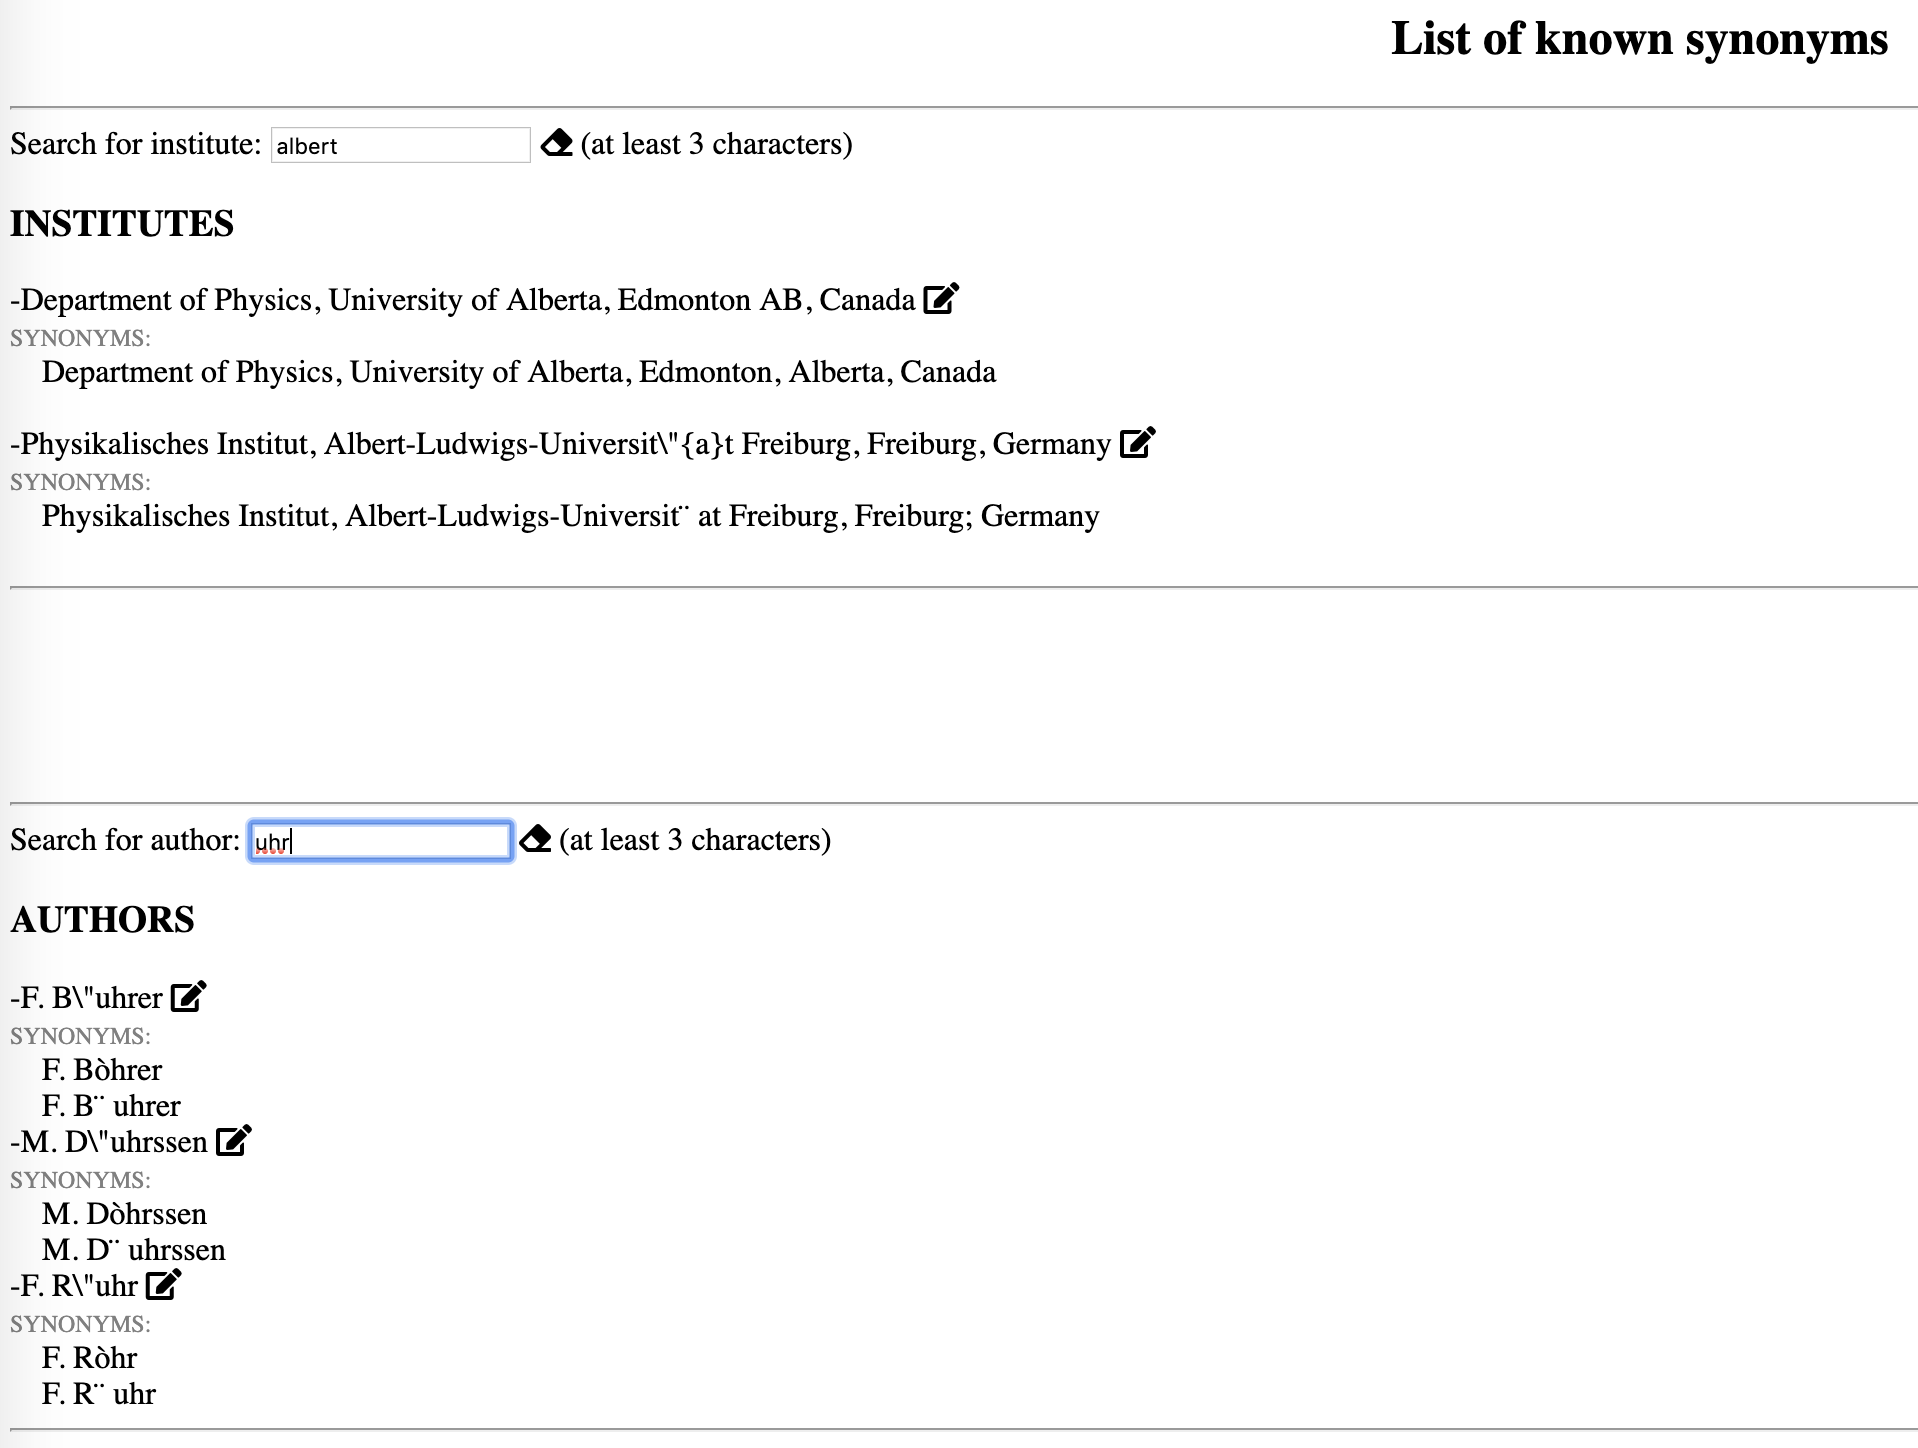
\includegraphics[width=0.9\textwidth]{figures/synonym_webpage.png}
  \caption{Proof checker synonyms’ webpage.}
  \label{fig:synonym_webpage}
\end{figure}

\subsubsection{Report page}
\label{sec:Report_page}
The proof checker provides a report after its run, one for each Paper and draft version. This report is provided and stored into a JSON file and must be parsed to show the report results into a human readable way. This is done by the proof$\_$report webpage (Fig.~\ref{fig:proof_report_webpage}).
On that report we can find all the paper information plus the real comparison results splitted by issue sections (see \ref{sec:app15}). The JSON file contains more information than what is displayed; this is done to allow the webpage to understand the correct way to show the huge amount of information and for future improvements. The webpage contains some “hidden” sections that are produced by the proof checker thanks to the known synonyms, and can be displayed by clicking on “Skipped +”. Here the page will show all the false positive results that the proof checker found on its comparison, but that are ignored thanks to the synonyms.
\begin{figure}[ht!]
  \centering
  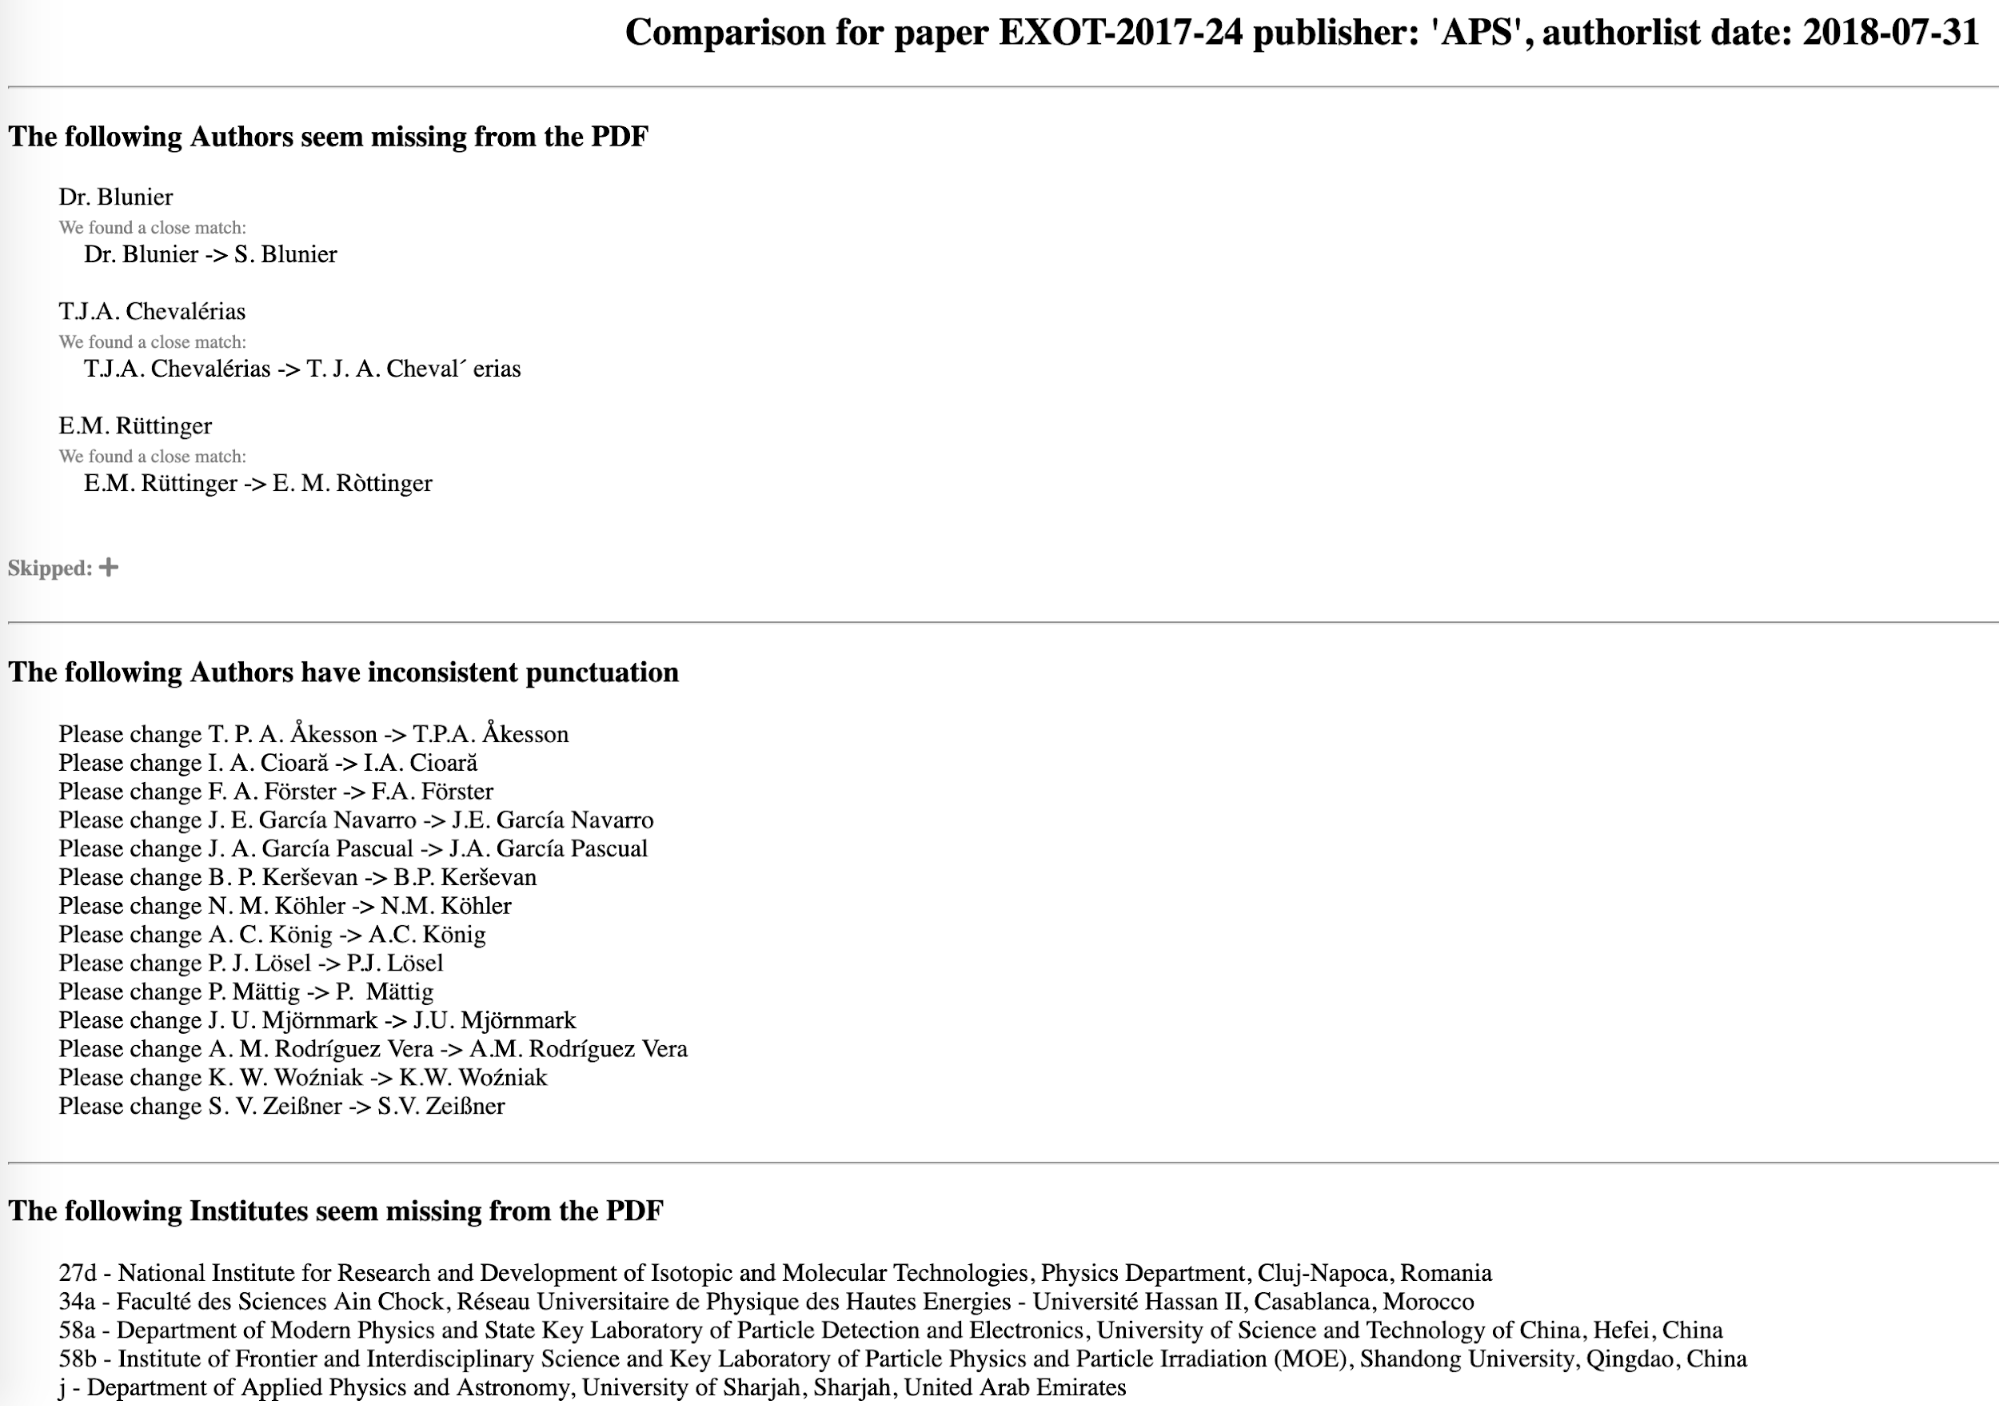
\includegraphics[width=0.9\textwidth]{figures/proof_report_webpage.png}
  \caption{Proof report webpage.}
  \label{fig:proof_report_webpage}
\end{figure}
The proof checker helps the Physics Office staff in a tedious task, but is way far from being a perfect tool. More than that, it will always need to be maintained and updated looking for new unexpected cases, changes on publication layouts, new conventions on the author lists and their format. A list of further improvements are in developers’ agenda, with the goal of having the user manually checking just a couple of dozens of cases instead of facing the list of hundreds of false positive they were used to until 2017.     
